\sloppy
\chapter{Aplicație software}
\label{chap:ch4}

\par
Capitolul de față descrie aplicația software realizată, prezentând structura sa generală, principalele componente și modul în care acestea comunică pentru a oferi funcționalitățile propuse.
Sunt oferite detalii despre arhitectură și sunt explicate principalele funcționalități. 
Capitolul se încheie cu un scurt manual de utilizare, conceput să ghideze utilizatorul în folosirea aplicației. 

\section{Arhitectura aplicației}
\label{sec:ch4sec1}

Aplicația este alcătuită din 3 componente: interfața utilizator (frontend), partea de server (backend) și sistemul de recomandare. 
Aceste componente au roluri bine definite și comunică între ele pentru a asigura funcționarea aplicației.
Frontend-ul gestionează interacțiunea cu utilizatorul, backend-ul coordonează logica aplicației și accesul la date, iar sistemul de recomandare oferă sugestii pe baza datelor oferite de server.
Arhitectura, așa cum este prezentată în figura \ref{FigArchitectureDiagram}, prezintă structura modulară ce permite separarea clară a responsabilităților.

\begin{figure}[htbp]
	\centering
    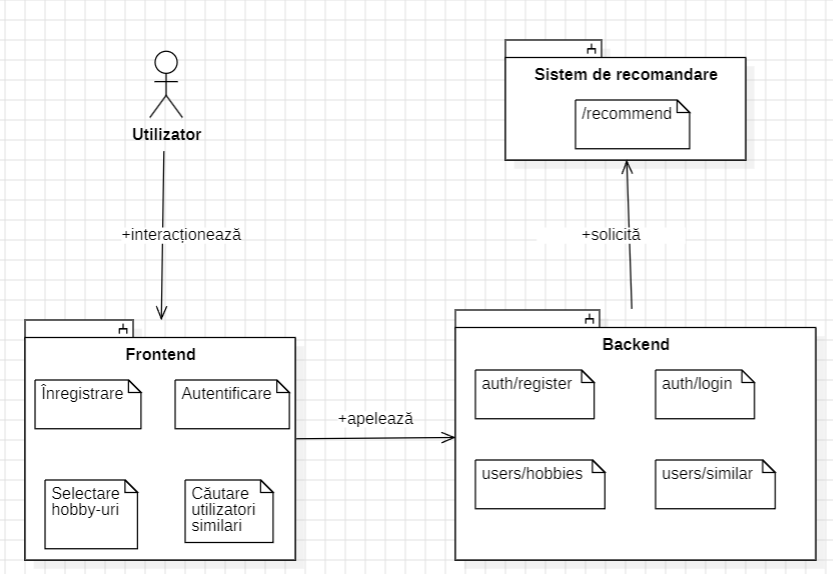
\includegraphics[scale=0.6]{./figures/architecture-diagram.png}
	\caption{Diagrama de arhitectură}
	\label{FigArchitectureDiagram}
\end{figure}

\subsection{Frontend}
\label{subsec:ch4sec1sub1}

Partea de frontend este dezvoltată în Ionic React \cite{ionicreactdocs}, tehnologie ce îmbină librăria React \cite{reactdocs}, scrisă în limbajul de programare JavaScript, 
utilizată pentru a construi interfețe utilizator și Ionic \cite{ionicdocs}, un instrument ce ajută la dezvoltarea aplicațiilor cross-platform. 
Folosind Ionic, aplicația poate fi instalată pe mai multe platforme --- web, mobile (Android, iOS), desktop --- utilizând același cod sursă. 
Această abordare eficientizează dezvoltarea și întreținerea aplicațiilor, permițând o experiență de utilizare uniformă, indiferent de dispozitiv folosit. 
\par
Interfața utilizator a aplicației este compusă din rute, pagini și componente. 
Paginile corespund unor ecrane complete din aplicație, iar componentele sunt părți reutilizabile ale aplicației, precum un formular sau buton personalizat.
Componentele primesc proprietăți și returnează elemente de interfață utilizator.
Rutele definesc ce pagină trebuie afișată atunci când utilizatorul accesează o anumită adresă (URL). 
De exemplu, ruta \texttt{/login} afișează pagina de autentificare, ruta \texttt{/register} afișează pagina de înregistrare ș.a.m.d.

\par
Frontend-ul comunică cu serverul prin apeluri HTTP, datele fiind transmise în formatul JSON.
În cadrul aplicației a fost creat fișierul \texttt{api.ts} care grupează toate cererile care sunt trimise către backend. 
Acest serviciu oferă funcții precum \texttt{register}, \texttt{login} și \texttt{saveHobbies}.
Aplicația folosește biblioteca Axios, o soluție populară și eficientă pentru manipularea cererilor HTTP.


\subsection{Backend}
\label{subsec:ch4sec1sub2}
Partea de server este scrisă în Java utilizând Spring Boot \cite{springbootdocs}, un instrument care ajută la simplificarea procesului de dezvoltare al aplicațiilor.
Acest framework permite crearea rapidă de API-uri REST, o integrare facilă cu baza de date și o organizare logică a codului în componente. Alegerea
acestei tehnologii a fost motivată de ecosistemul extins pe care îl oferă, configurarea redusă și structura modulară. 

\par
Proiectul este organizat conform principiilor arhitecturii stratificate, adaptate pentru o aplicație REST. 
Așadar, codul sursă este împărțit în mai multe directoare (pachete) care separă responsabilitățile logice: 
\begin{itemize}
    \item controller: include clase care gestionează cererile HTTP venite de la frontend. Acestea definesc rutele API și interacționează direct cu serviciile.
    \item service: conține implementările operațiilor specifice fiecărei funcționalități (înregistrare utilizator, adăugare hobby etc.). Acest strat realizează legătura între controller și repository. 
    \item repository: definește interfețe care extind \texttt{JpaRepository}. Acestea se concentrează asupra operațiilor CRUD (Create, Read, Update, Delete) cu efect direct asupra bazei de date.
    \item domain: conține entitățile din domeniul aplicației. Acestea sunt adnotate cu specificații precum \texttt{@Entity}, \texttt{@Table} etc. pentru a le asocia tabelelor din baza de date.
\end{itemize}  
Pe lângă aceste pachete clasice, proiectul include și alte componente utile:
\begin{itemize} 
    \item dto (Data Transfer Object): conține clase care precizează formatul datelor transmise între client și server.
    \item mapper: cuprinde clase cu metode statice folosite la conversia obiectelor de tip domeniu în obiecte de tip DTO și vice-versa.
    \item exception: definește clase care se ocupă de tratarea erorilor. Acestea extind clasa \texttt{Exception} cu scopul de a crea excepții personalizate.
    \item security: gestionează autentificarea și autorizarea. Oferă implementare pentru JWT (Json Web Token).
\end{itemize}
\subsubsection*{Model de date}
Entitățile de bază ale aplicației sunt User, Hobby și HobbyType. Fiecare dintre acestea sunt reprezentate printr-o clasă Java, asociată unei tabele din baza de date.
În figura \ref{FigClassDiagram} sunt definite clar relațiile între obiecte.

\begin{figure}[htbp]
	\centering
    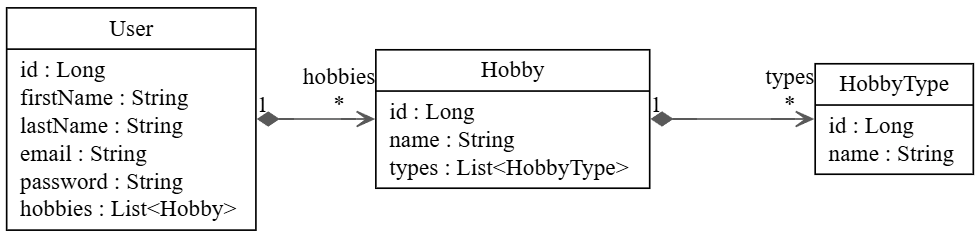
\includegraphics[scale=0.45]{./figures/class-diagram.png}
	\caption{Diagrama de clase}
	\label{FigClassDiagram}
\end{figure}

\subsubsection*{Baza de date}
Conectarea la baza de date se face cu ajutorul fișierului de configurare \texttt{application.properties}, unde sunt specificate datele de acces precum URL, utilizator și parolă. 
Baza de date folosită este PostgreSQL \cite{postgresqldocs}, consacrată pentru fiabilitate și performanță. 
Pentru asocierea obiectelor Java cu tabelele bazei de date s-a utilizat Java Persistence API împreună cu framework-ul Hibernate \cite{hibernatedocs}, permițând manipularea entităților Java ca tabele din baza de date, așa cum se poate vedea în figura \ref{FigDbDiagram}.

\begin{figure}[htbp]
	\centering
    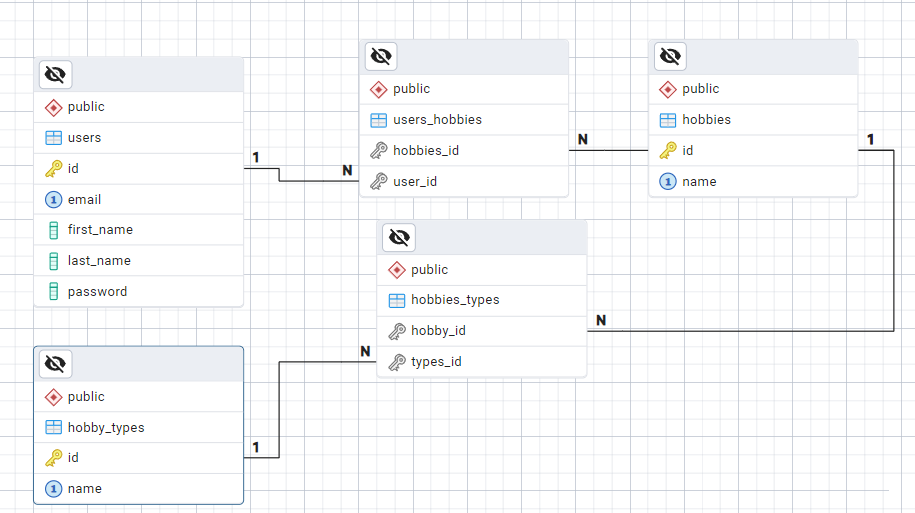
\includegraphics[scale=0.65]{./figures/db-diagram.png}
	\caption{Diagrama bazei de date}
	\label{FigDbDiagram}
\end{figure}

\subsubsection*{Securitate}
Aplicația implementează câteva mecanisme minimale de asigurare a securității și de protejare a accesului la resursele interne.
În ceea ce privește parola asociată contului, aceasta este stocată sub formă criptată, folosind algoritmul BCrypt, iar pentru siguranța parolei, aplicația impune o lungime minimă de 8 caractere a acesteia.
Atunci când utilizatorul se autentifică cu succes, primește un JSON Web Token (JWT). Acest token este folosit pentru identificarea ulterioară a utilizatorului în cererile către server.
Deoarece majoritatea rutelor din aplicație sunt restricționate, utilizatorul are nevoie de un token valid pentru a le accesa, ceea ce asigură un control al accesului la funcționalitățile interne ale aplicației.

\subsection{Sistemul de recomandare}
\label{subsec:ch4sec1sub3}
Pentru a determina gradul de similaritate între utilizatori pe baza hobby-urilor comune, sistemul folosește coeficientul de similaritate Jaccard.
Această metodă compară seturile de hobby-uri ale fiecărui utilizator și calculează raportul dintre elementele comune și totalitatea elementelor distincte din cele două seturi, rezultând o valoare reală între 0 și 1.
Metoda este simplă și intuitivă, fiind adecvată pentru compararea mulțimilor neordonate de termeni.
Implementarea funcției care calculeaza similaritatea Jaccard este prezentată în secvența de cod \ref{CodeJaccard}.
\par
Principalele argumente care au stat la baza alegerii acestei modalități de calcul al similarității sunt eficiența sa computațională, prin faptul că nu necesită resurse mari de calcul, dar și compatibilitatea sa cu datele binare, precum cele legate de hobby-uri (un hobby poate să fie prezent sau absent).
De asemenea, există o simetrie în relația dintre utilizatori: similaritatea dintre utilizatorul A și B este aceeași cu cea dintre utilizatorul B și A, favorizând constituirea unei rețele coerente între persoane.

\begin{lstlisting}[caption={Algoritmul de calcul al similarității Jaccard}, label={CodeJaccard}]
def jaccard_similarity(set1, set2):
    if not set1 or not set2:
        return 0.0
    intersection = len(set1.intersection(set2))
    union = len(set1.union(set2))
    return intersection / union
\end{lstlisting}    

\subsubsection*{Setul de date}
Pentru a popula baza de date cu o listă de hobby-uri cât mai bogată și realistă, s-au fuzionat trei seturi de date disponibile pe platformele Kaggle \cite{kaggle_Raj, kaggle_dawid} și HuggingFace \cite{hf_Ugurcan}.
După îmbinarea acestora, a fost nevoie de o prelucrare atentă a setului de date pentru a standardiza formatul.
Numele hobby-urilor au fost normalizate, iar în cazul în care au apărut duplicate, acestea au fost eliminate, însă tipurile lor au fost comasate.
Tipurile hobby-urilor au fost la rândul lor prelucrate, deoarece erau exprimate inconsistent, separate fie prin virgulă, fie prin conjuncția ”and”, iar duplicatele au fost excluse.
În urma procesării, s-a obținut un set de aproximativ 730 de hobby-uri care a fost introdus în baza de date pentru ca utilizatorii să poată selecta hobby-urile dintr-o listă structurată.

\subsubsection*{Comunicare cu serverul Java}
Recomandările se realizează printr-o comunicare între serverul Java și sistemul de recomandare, care este implementat separat, scris în Python, folosind framework-ul Flask \cite{flaskdocs}.
Acest serviciu extern este responsabil cu procesarea datelor și calculul gradului de asemănare.
Atunci când utilizatorul accesează pagina de căutare a recomandărilor, aplicația trimite către serverul Python informații despre hobby-urile acestuia, precum și despre restul utilizatorilor existenți.
Sistemul analizează datele și returnează o listă de utilizatori cu interese comune, ordonați în funcție gradul de similaritate.
\par
Alegerea de a implementa separat acest sistem de recomandare a fost motivată de dorința de a păstra componenta independentă față de restul aplicației.
Această abordare dă posibilitatea de a reutiliza codul într-un alt context, precum recomandarea de produse, cărți sau filme.

\section{Funcționalități}
\label{sec:ch4sec2}

Aplicația se concentrează asupra a patru acțiuni esențiale: înregistrarea unui cont, autentificarea unui utilizator, selectarea hobby-urilor dorite și căutarea altor utilizatori cu hobby-uri similare.
Diagrama din figura \ref{FigUseCaseDiagram} evidențiază aceste funcționalități.

\begin{figure}[htbp]
	\centering
    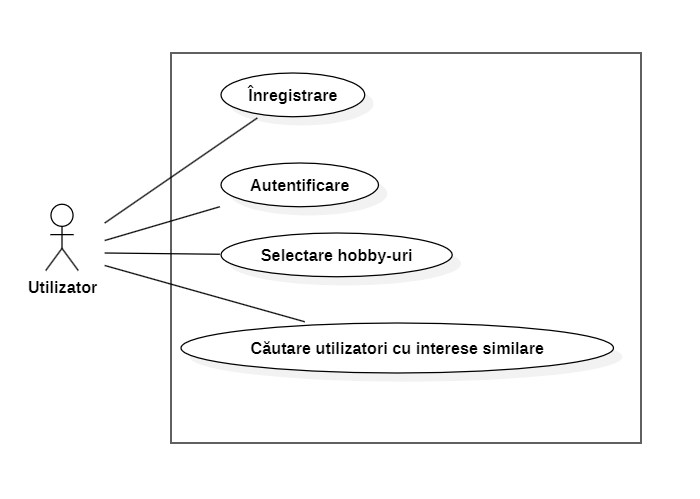
\includegraphics[scale=0.60]{./figures/usecase-diagram.png}
	\caption{Diagrama cazurilor de utilizare}
	\label{FigUseCaseDiagram}
\end{figure}

\subsection{Cerințe funcționale}
\label{subsec:ch4sec2sub1}

\subsubsection*{Înregistrarea utilizatorului}
Această funcționalitate permite unui user nou să își creeze cont în aplicație. Pagina conține un formular cu câmpurile: nume, prenume, email sau parolă.
La acționarea butonului Register, aplicația validează datele scrise de utilizator, iar în cazul în care
nu există erori, trimite o cerere HTTP de tip POST către endpoint-ul \texttt{/auth/register} expus de backend. În caz contrar, programul oferă user-ului feedback imediat prin mesaje de eroare sugestive.
Pe backend, datele se revalidează pentru a asigura securitatea și integritatea acestora. 
Contul utilizatorul se salvează în baza de date doar dacă nu există deja unul cu aceeași adresă de email, altfel se aruncă o excepție corespunzătoare.
Serverul trimite răspuns, după caz, fie datele user-ului creat, fie un mesaj de eroare.

\subsubsection*{Autentificarea utilizatorului}
Pentru a accesa restul funcționalităților, utilizatorul trebuie să se autentifice. Pagina dedicată logării cuprinde un formular cu două câmpuri: adresa de email și parolă.
În urma apăsării butonului Login, aplicația validează local datele introduse. În lipsa erorilor, se inițiază o cerere HTTP POST către endpoint-ul \texttt{/auth/login}.
Pe partea de server, datele se verifică din nou, iar dacă acestea sunt corecte și corespund unui cont existent, se trimite un răspuns ce conține datele utilizatorului logat și un token JWT generat.
În cazul unor date invalide (parolă incorectă, email inexistent), sistemul oferă un mesaj de eroare specific. După autentificare, token-ul JWT este stocat, iar utilizatorul este redirecționat către pagina principală.


\subsubsection*{Alegerea hobby-urilor}
După ce utilizatorul este autentificat, aplicația verifică dacă acesta are hobby-uri. Dacă nu sunt identificate hobby-uri pentru user-ul logat, programul prezintă
ecranul de alegere a hobby-urilor. Acesta conține un buton pentru salvare, o bară de căutare și listă de componente ce afișează numele și tipul fiecărui hobby, alături de un checkbox.
Lista hobby-urilor este primită de la server prin intermediul unui apel HTTP de tip GET către endpoint-ul \texttt{/users/hobbies}. 
Utilizatorul poate filtra lista după numele hobby-urilor folosind bara de căutare. 
După ce user-ul selectează hobby-urile dorite și apasă butonul Save, se trimite o cerere HTTP de tip POST pentru a salva hobby-urile selectate.

\subsubsection*{Căutarea utilizatorilor cu hobby-uri similare}
Dacă s-au găsit hobby-uri pentru utilizatorul autentificat, atunci aplicația afișează pagina de căutare a utilizatorilor cu hobby-uri asemănătoare.
Aceasta prezintă un buton pentru căutare cu nume sugestiv. 
La apăsarea acestuia se trimite o cerere HTTP către endpoint-ul \texttt{/users/similar}.
Backend-ul creează o listă cu ID-urile tutoror utilizatorilor și hobby-urile acestora, din care se elimină utilizatorul logat.
Această listă și utilizatorul logat se transmit sistemului de recomandare, printr-o metodă HTTP către endpoint-ul \texttt{/recommend}.
Sistemul de recomandare calculează similaritatea hobby-urilor dintre utilizatorul logat și ceilalți utilizatori și returnează ca răspuns lista de ID-uri ale utilizatorilor recomandați, memorând pentru fiecare un scor al potrivirii.
Partea de server primește de la sistemul de recomandare lista sortată descrescător după acel scor. 
Pe baza fiecărui ID din listă, programul caută informațiile legate de utilizator (nume, e-mail și hobby-urile), pe care le asociază cu scorul primit.
Lista completă este transmisă interfeței utilizator pentru afișare.
Utilizatorului logat i se vor prezenta utilizatorii recomandați, vizualizând pentru fiecare numele, e-mailul, lista hobby-urilor și scorul similarității.


\subsection{Cerințe nefuncționale}
\label{subsec:ch4sec2sub2}
Pe lângă funcționalitățile oferite utilizatorului, sistemul proiectat trebuie să respecte o serie de cerințe nefuncționale care asigură calitatea generală a produsului.
Referitor la interfața utilizator, aceasta trebuie să fie intuitivă și ușor de utilizat pentru a se putea adresa unui număr mare de utilizatori.
În plus, aplicația trebuie să fie portabilă datorită faptului că este construită cu ajutorul framework-ului Ionic.
De asemenea, cerințele impun ca sistemul să aibă un mecanism robust de securitate în care accesul la funcționalitățile interne ale aplicației să fie restricționate și autorizate doar în prezența unor token-uri valide. 
În cele din urmă, se dorește ca aplicația să fie scalabilă, ușor de întreținut și de actualizat, pentru a permite extinderea funcționalităților în viitor. 


\section{Manual de utilizare}
\label{sec:ch4sec3}

La prima interacțiune cu aplicația, utilizatorul are acces la două ecrane, la cel de logare și la cel de înregistrare. 
În funcție de calitatea user-ului (nou sau înregistrat) poate alege să se înregistreze sau să se autentifice.
\par
Pentru a se loga, utilizatorul trebuie să introducă email-ul și parola cu care s-a înregistrat în prealabil, așa cum se poate vedea în figura \ref{FigLoginPage}. 
La apăsarea butonului de autentificare, sistemul verifică datele și redirecționează utilizatorul către pagina principală sau notifică cu privire la erorile apărute. 

\begin{figure}[htbp]
	\centering
    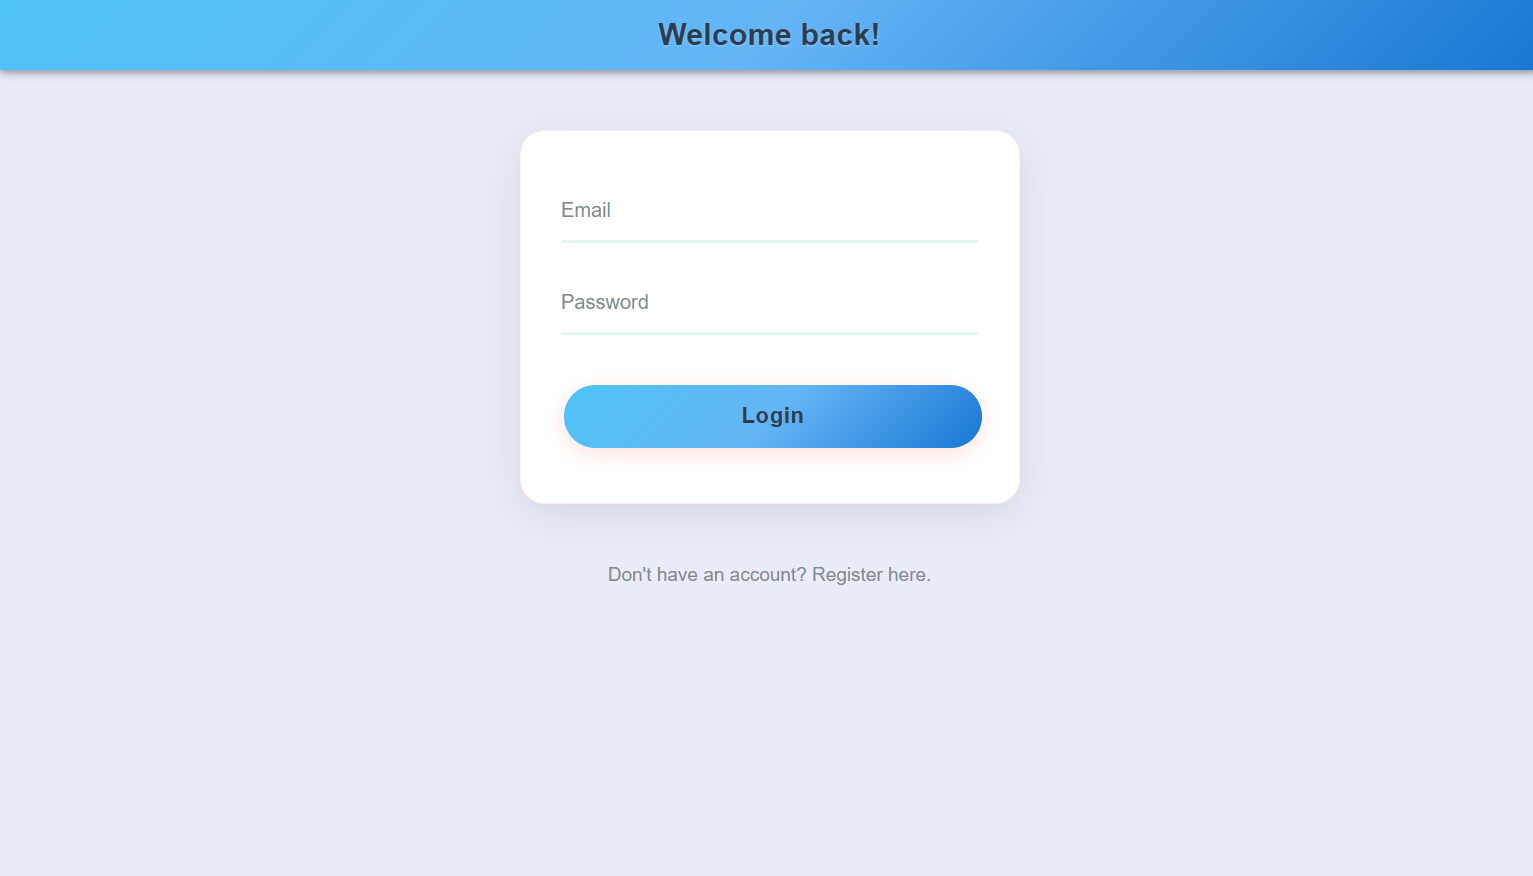
\includegraphics[scale=0.35]{./figures/login-page.png}
	\caption{Pagina de autentificare}
	\label{FigLoginPage}
\end{figure}

\par
Figura \ref{FigRegisterPage} ilustrează pagina de înregistrare, unde utilizatorul trebuie să completeze formularul cu numele, adresa de e-mail și parola.
La acționarea butonului de înregistrare, sistemul validează informațiile furnizate și creează contul utilizatorului sau afișează mesaje corespunzătoare în cazul unei erori.
După o înregistrare cu succes, user-ul este redirecționat către pagina de logare.

\begin{figure}[htbp]
	\centering
    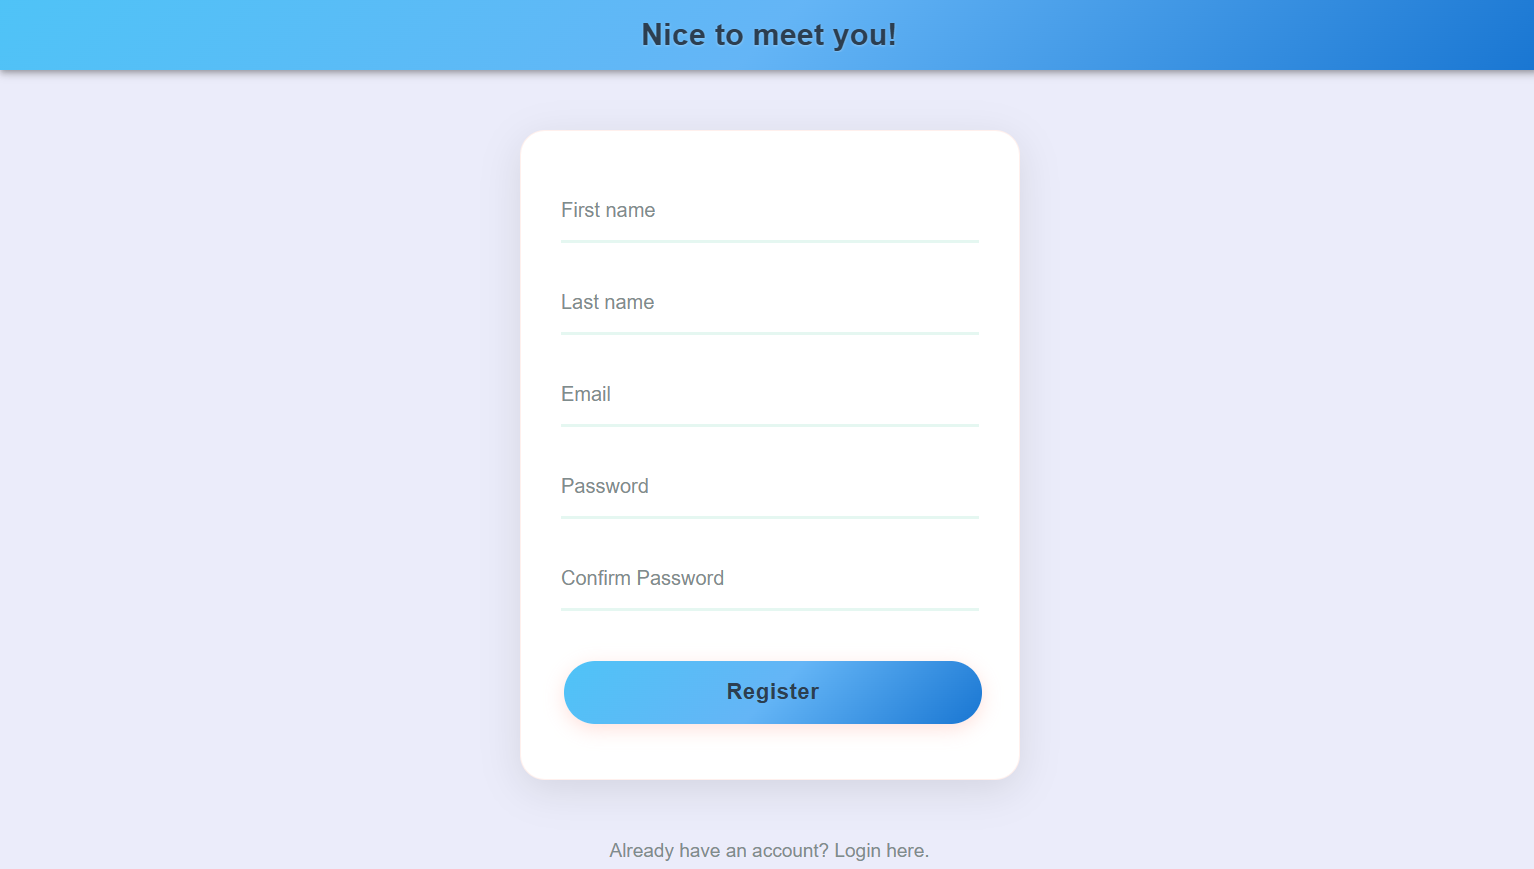
\includegraphics[scale=0.35]{./figures/register-page.png}
	\caption{Pagina de înregistrare}
	\label{FigRegisterPage}
\end{figure}

\par
În cazul în care utilizatorul logat nu are adăugate hobby-uri, un ecran dedicat acestei acțiuni va fi afișat imediat după logare, așa cum se poate observa în figura \ref{FigOnboardingPage}.
Aici user-ul poate alege din lista de hobby-uri existente, prin intermediul unui checkbox. 
De asemenea, hobby-urile pot fi filtrate după nume, folosind bara de căutare.
După selectare, acestea pot fi salvate prin apăsarea butonului Save.

\begin{figure}[htbp]
	\centering
    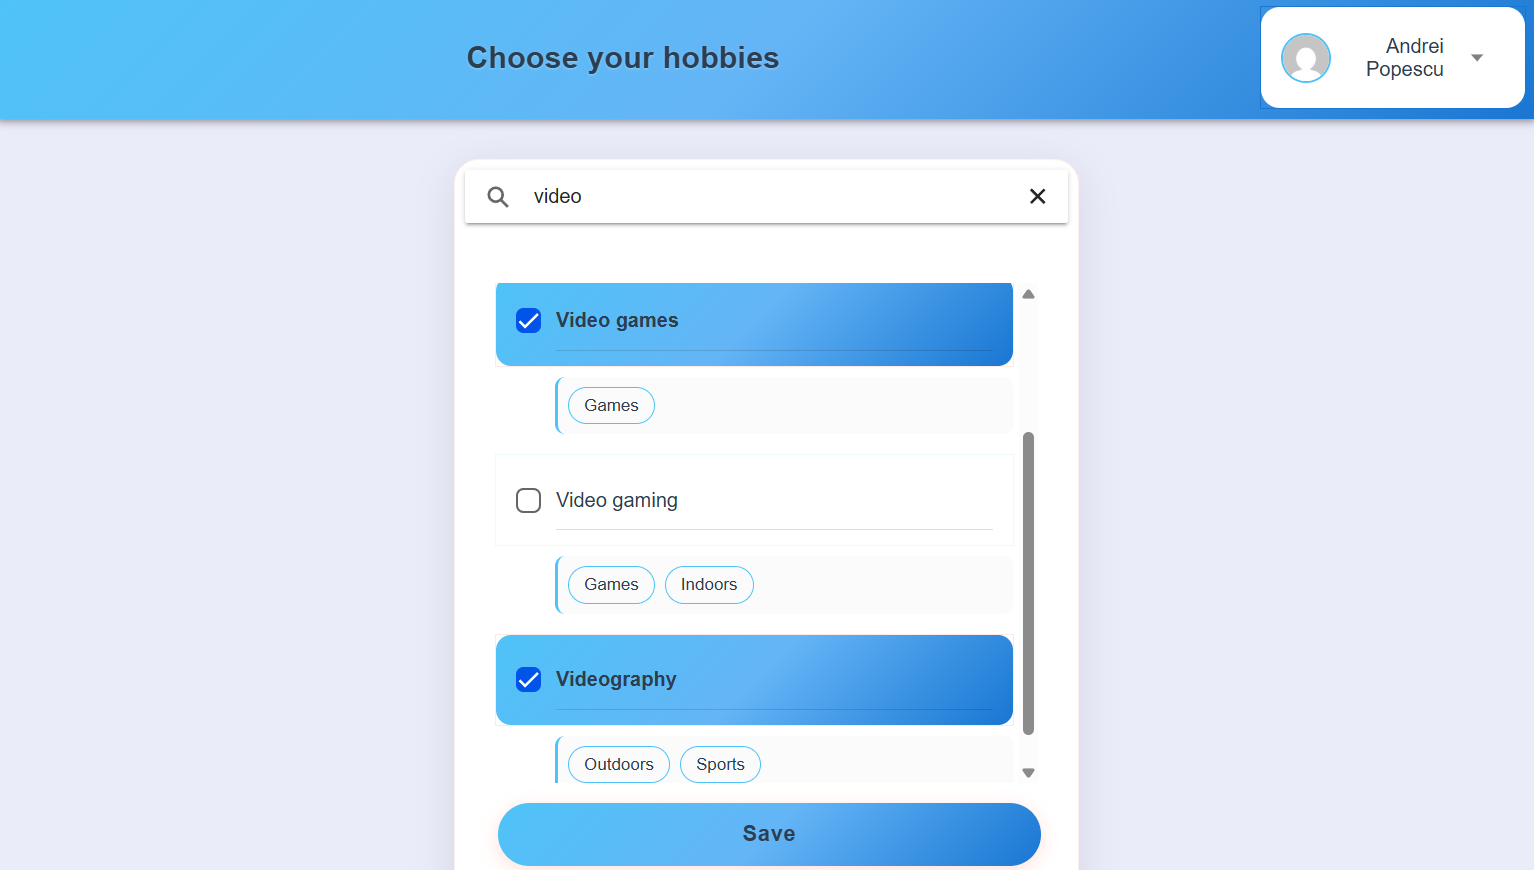
\includegraphics[scale=0.35]{./figures/onboarding-page.png}
	\caption{Pagina afișată utilizatorilor fără hobby-uri selectate}
	\label{FigOnboardingPage}
\end{figure}

\par
Dacă utilizatorul logat are hobby-uri selectate, se prezintă pagina de căutare a utilizatorilor cu hobby-uri asemănătoare, conform figurii \ref{FigHomePage}.
Pentru căutare, user-ul apasă butonul dedicat de pe ecran și se afișează lista utilizatorilor recomandați.
Această listă este ordonată descrescător după scorul potrivirii.

\begin{figure}[htbp]
	\centering
    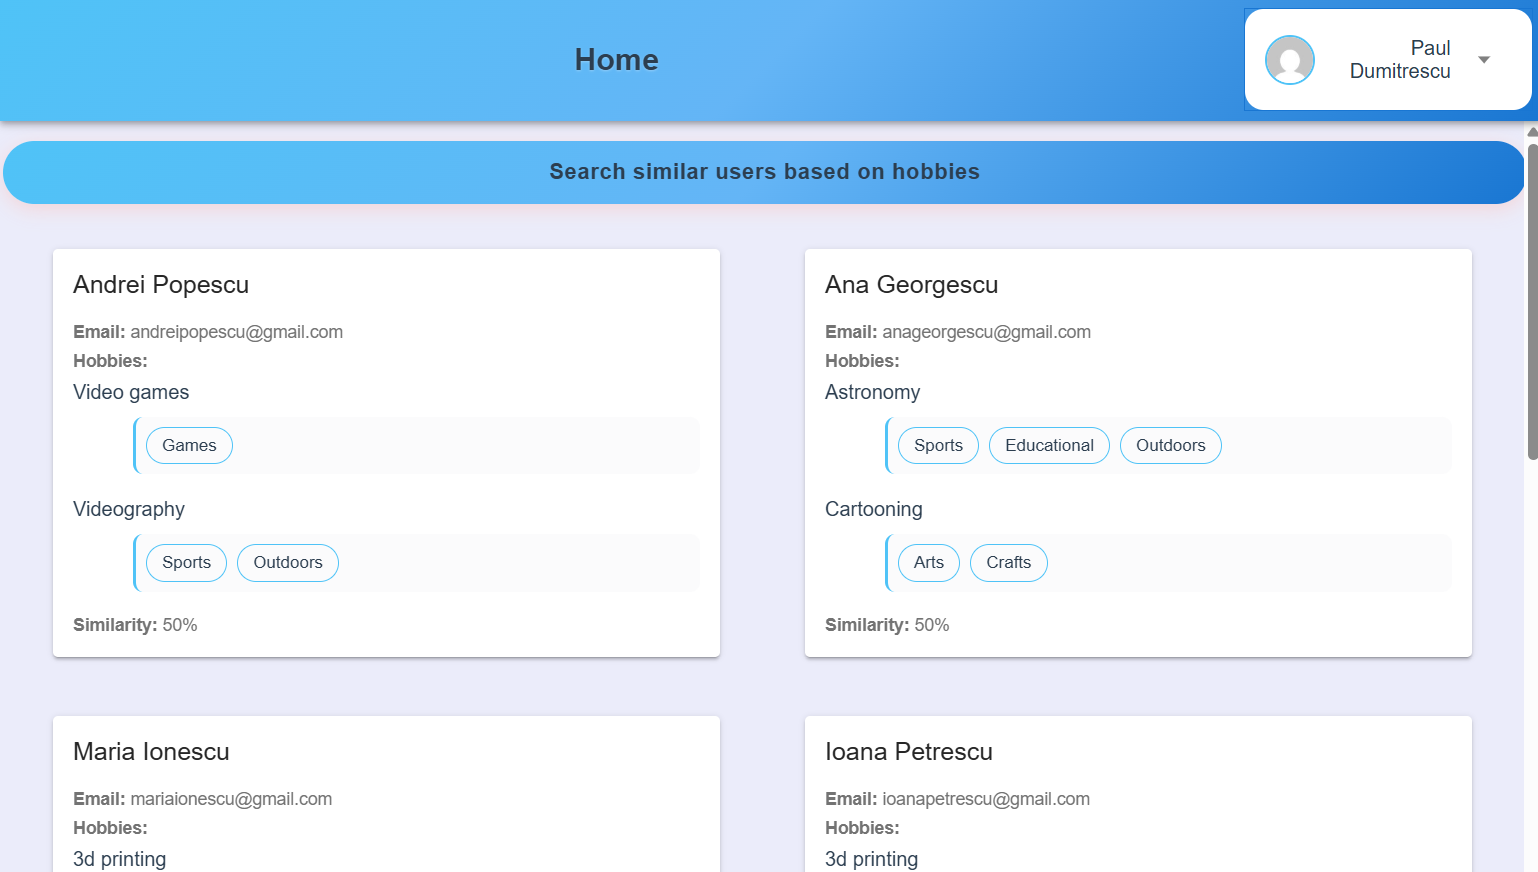
\includegraphics[scale=0.35]{./figures/home-page.png}
	\caption{Pagina de căutare a utilizatorilor cu interese comune}
	\label{FigHomePage}
\end{figure}

\par
De asemenea, utilizatorul se poate deconecta din aplicație. La apăsarea butonului ilustrat în figura \ref{FigLogoutButton}, user-ul va fi redirecționat către pagina de autentificare.

\begin{figure}[htbp]
	\centering
    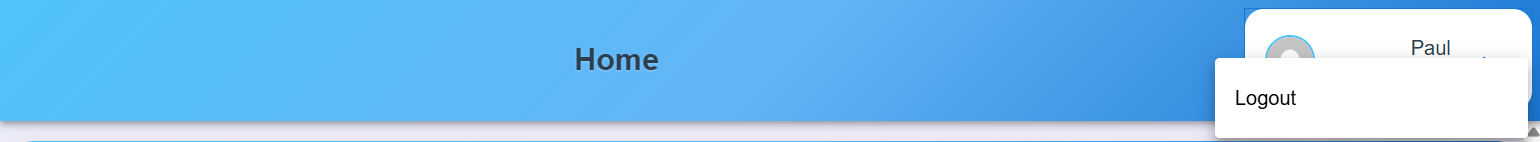
\includegraphics[scale=0.35]{./figures/logout-component.png}
	\caption{Deconectarea utilizatorului}
	\label{FigLogoutButton}
\end{figure}

\section{Testare și validare}
\label{sec:ch4sec4}
Pentru validarea funcționalităților aplicației dezvoltate, aceasta a fost testată pe platforma web, utilizând browsere precum Chrome și Brave.
Deși framework-ul Ionic oferă posibilitatea de a rula aplicația și pe alte platforme (mobile și desktop), testarea s-a concentrat pe web.
Procesul de testare a cuprins verificarea aplicației în întregime, cu asigurarea că toate scenariile de utilizare au fost luate în calcul. 

\subsection{Metodologia de testare}
\label{subsec:ch4sec2sub1}
\subsubsection*{Testare manuală}
Această abordare a implicat testarea sistematică a întregii aplicații prin interacțiunea directă cu interfața.
Fiecare funcționalitate a fost testată individual pentru a asigură că este întocmai cu specificațiile: procesul de înregistrare și autentificare, adăugarea hobby-urilor, generarea recomandărilor și navigarea prin diferitele secțiuni ale aplicației.
Au fost testate atât cazurile de utilizare standard cât și scenariile de eroare pentru a verifica comportamentul în situații limită.
\subsubsection*{Testare de interfață}
Această metodă s-a concentrat pe evaluarea caracteristicilor vizuale și a experienței utilizatorului.
Au fost verificate elementele de design din întreaga aplicație și modul în care interfața răspunde la schimbările de dimensiune ale ecranului.
Suplimentar, s-a verificat funcționarea corectă a elementelor interactive și consistența tranzițiilor între pagini.

\subsection{Scenarii de testare}
\label{subsec:ch4sec2sub2}
Pentru validarea aplicației prin testare manuală, au fost create și executate mai multe scenarii de testare care acoperă toate funcționalitățile sistemului.
Scenariile au fost împărțite în două categorii: scenarii pozitive, care testează comportamentul normal al aplicației, și scenarii negative, care verifică reacția programului la situații excepționale.
Fiecare dintre aceste scenarii a fost executat prin navigarea manuală în aplicație.
Printre scenariile testate se numără: înregistrarea unui utilizator nou prin completarea formularului cu date valide și invalide, autentificarea unui utilizator cu credențiale corecte și incorecte, adăugarea hobby-urilor și generarea recomandărilor pentru diferite profiluri de utilizator.
Această modalitate de testare a avut scopul de a identifica principalele erori ale funcționalităților și problemele legate de utilizabilitate și experiența utilizatorului.

\subsection{Rezultate}
\label{subsec:ch4sec2sub3}
Procesul de testare manuală a surprins funcționarea corectă a majorității funcționalităților.
Aplicația gestionează corect atât cazurile de succes cât și cele de eroare.
Datorită mesajelor clare de eroare pe care sistemul le afișează utilizatorilor, aceștia pot remedia ușor situațiile în care apar probleme.
În linii mari, testarea a confirmat faptul că aplicația răspunde cerințelor funcționale și nefuncționale stabilite anterior.

\subsection{Limitări și îmbunătățiri}
\label{subsec:ch4sec2sub4}
Deși procesul de verificare a validat sistemul proiectat, au fost identificate limitări ale acestor metode.
Multitudinea de cazuri de testare și combinațiile scenariilor fac ca această practică să fie dificilă și susceptibilă la erori umane.
În plus, pe măsură ce aplicația crește, testarea manuală devine consumatoare de timp și greu de gestionat.
Ca modalități de îmbunătățire, se recomandă implementarea unui sistem de testare automată și includerea celorlalte platforme în scenariile de testare.